\chapter{Implementation}\label{cha:implementation}

	Main focus of this chapter is on development and its progress. It describes application structure, its layers, used
	principles, design patterns and conventions taking the analytical part into account.

	\section{Environment and new Spring Roo project setup}
	
	\subsection{Development platform}\label{cha:implementation:platform}
	
	It is not a secret that developing applications for Java platform is resource consuming and requires solid performance
	for effective work. Luckily today's computers provide good computing power since mid-level price range and purchasing
	multi-core CPU and several GB of RAM is a standard.
	
	My configuration during development and writing this master's thesis was:
	
	\begin{itemize}
		\item Dell Latitude E6410 laptop
		\item CPU Intel Core i5 Quad Core @ 2.5GHz
		\item 4GB RAM DDR3
		\item 120GB SSD MLC hard drive 
	\end{itemize}
	
	What is more important these days is developer's software equipment. Starting with OS, 64bit is a must. It depends on
	a personal preference to use IDE or not and then of course various support tools like console or term emulator,
	monitoring tools, \ldots

	This is what I have been using:	

	\begin{itemize}
		\item Windows 7 64bit, openSUSE 12.2 64bit
		\item Java 7 runtime  and compile (Oracle's JDK 1.7.0\_10)
		\item Maven 3.0.3
		\item Cygwin 1.7.10 with Bash as a primary shell in Console2
		\item Spring Roo 1.2.2 with Java 1.7 support
		\item Eclipse IDE, 3.7.2 Indigo and 4.2.1 Juno
		\begin{itemize}
			\item Spring STS
			
			Spring Roo's installation path needs to be set up.
			\item JBoss Tools  
			
			Maven tool should be switched from Eclipse's embedded implementation to the system wide installed one.
		\end{itemize}
	\end{itemize}
	
	To make all this work, it is required to set up system environment variables properly. Especially:
	
	\begin{itemize}
		\item JAVA\_HOME
		
		Pointing to the JDK 7 installation directory.
		\item MAVEN\_HOME
		
		Pointing to the Maven 3 installation directory.
		\item ROO\_HOME
		
		Pointing to the Spring Roo 1.2 installation directory.
		\item append all the above concatenated with \textbf{/bin} to the \textbf{PATH} variable 
	\end{itemize}
	
	After all these steps are done, nothing should stand in the way anymore and development can start straight ahead.
	
	\subsection{Configuring the new project}
	
	RESTful API is using Maven and Spring Roo, which play very nicely together. I could either use basic Maven's
	\verb|archetype|\footnote{A template used by Maven to create a new project.} and configure the project for Spring Roo
	or let it create standard Spring Roo project and tweak it, as I do not want a standard web project, but Spring Roo
	without Spring MVC's View integrated with Apache CXF.
	
	In the end, I decided to combine both approaches. Because basic Maven project is nothing else but a standard directory
	structure with JEE web application and Maven configuration files, this gives me a clean start. On the other hand,
	Spring Roo will create a sample web project (also Maven project), from which I will simply take what I need in my clean
	Maven project to make it play with Spring Roo.
	
	Let's create basic Maven project first via Eclipse IDE - no archetype:
	
	\begin{verbatim}
		.
	|-- pom.xml
	|-- src
	|   |-- main
	|   |   |-- java
	|   |   `-- resources
	|   `-- test
	|       |-- java
	|       `-- resources
	`-- target
	    |-- classes
	    |   `-- META-INF
	    |       `-- MANIFEST.MF
	    `-- test-classes
	
	11 directories, 2 files
	\end{verbatim}
	
	Explanation of the above follows:
	
	\begin{itemize}
		\item \textbf{pom.xml} 
		
		Maven's configuration file for this project. Contains project's metadata (name, description, identification, \ldots)
		and what is important - dependencies, plugins, reports and their various settings.
		\item \textbf{src/main/java}
		
		Standard place for Java source code.
		\item \textbf{src/main/resources}
		
		A place for various resources like metadata, configuration files, \ldots This directory will be in classpath at
		runtime.
		\item \textbf{src/test/java}
		
		Standard place for test Java source code. Unit and integration tests are placed here.
		\item \textbf{src/test/resources}
		
		Its role is the same as of \textbf{src/main/resources} directory, but this one is in classpath only during test
		phase.
		\item \textbf{target}
		
		Build directory and temporary directory. This is where all Maven outputs including deployable archive or report
		results are written. During the development process can be simply ignored.
	\end{itemize}
	
	How different from basic Maven project Spring Roo's project is? Let's create it by using Roo Shell take a look:
	
	\begin{verbatim}
	$ mkdir MI-MPR-DIP-Admission-Roo
	$ cd MI-MPR-DIP-Admission-Roo
	$ roo.sh
	    ____  ____  ____
	   / __ \/ __ \/ __ \
	  / /_/ / / / / / / /
	 / _, _/ /_/ / /_/ /
	/_/ |_|\____/\____/    1.2.1.RELEASE [rev 6eae723]
	
	
	Welcome to Spring Roo. For assistance press TAB or
	type "hint" then hit ENTER.
	roo> project --topLevelPackage cz.cvut.fit.mi_mpr_dip.admission
	Created ROOT\pom.xml
	Created SRC_MAIN_RESOURCES
	Created SRC_MAIN_RESOURCES\log4j.properties
	Created SPRING_CONFIG_ROOT
	Created SPRING_CONFIG_ROOT\applicationContext.xml
	roo>
	\end{verbatim}
	
	Which will create a new Roo project with this structure:
	
	\begin{verbatim}
		.
	|-- log.roo
	|-- pom.xml
	`-- src
	    `-- main
	        `-- resources
	            |-- META-INF
	            |   `-- spring
	            |       `-- applicationContext.xml
	            `-- log4j.properties
	
	5 directories, 4 files
	\end{verbatim}
	
	It created basic Maven project structure, with basic Spring context setup, \verb|log4j|\footnote{Very popular and
	still widely used logging library, but there are already better implementations available. Log4j is quite an old
	library, development is discontinued and using facade SLF4J with Logback as an implementation is a standard nowadays.
	This is why I am going to replace it in RESTful API.} configuration and pom.xml contains all necessary dependencies.
	
	Let's use some more of Roo's features:
	
	\begin{verbatim}
	roo> jpa setup --provider HIBERNATE \
	--database HYPERSONIC_IN_MEMORY
	Created SPRING_CONFIG_ROOT\database.properties
	Updated SPRING_CONFIG_ROOT\applicationContext.xml
	Created SRC_MAIN_RESOURCES\META-INF\persistence.xml
	Updated ROOT\pom.xml
	...
	roo>
	\end{verbatim}
	
	The above just added persistence capabilities to the project via JPA. I know that root if the entire RESTful API is an
	admission, which will also serve as a key domain object - a Person is 1:1 related to the Admission. Thus I will create
	Admission domain object via Roo Shell:
	
	\begin{verbatim}
	roo> entity jpa --class ~.domain.Admission --testAutomatically
	Created SRC_MAIN_JAVA\cz\cvut\fit\mi_mpr_dip\admission
	\domain
	Created SRC_MAIN_JAVA\cz\cvut\fit\mi_mpr_dip\admission
	\domain\Admission.java
	Created SRC_TEST_JAVA\cz\cvut\fit\mi_mpr_dip\admission
	\domain
	Created SRC_TEST_JAVA\cz\cvut\fit\mi_mpr_dip\admission
	\domain\AdmissionDataOnDemand.java
	Created SRC_TEST_JAVA\cz\cvut\fit\mi_mpr_dip\admission
	\domain\AdmissionIntegrationTest.java
	Created SRC_MAIN_JAVA\cz\cvut\fit\mi_mpr_dip\admission
	\domain\Admission_Roo_Configurable.aj
	Created SRC_MAIN_JAVA\cz\cvut\fit\mi_mpr_dip\admission
	\domain\Admission_Roo_Jpa_Entity.aj
	Created SRC_MAIN_JAVA\cz\cvut\fit\mi_mpr_dip\admission
	\domain\Admission_Roo_Jpa_ActiveRecord.aj
	Created SRC_MAIN_JAVA\cz\cvut\fit\mi_mpr_dip\admission
	\domain\Admission_Roo_ToString.aj
	Created SRC_TEST_JAVA\cz\cvut\fit\mi_mpr_dip\admission
	\domain\AdmissionDataOnDemand_Roo_Configurable.aj
	Created SRC_TEST_JAVA\cz\cvut\fit\mi_mpr_dip\admission
	\domain\AdmissionDataOnDemand_Roo_DataOnDemand.aj
	Created SRC_TEST_JAVA\cz\cvut\fit\mi_mpr_dip\admission
	\domain\AdmissionIntegrationTest_Roo_Configurable.aj
	Created SRC_TEST_JAVA\cz\cvut\fit\mi_mpr_dip\admission
	\domain\AdmissionIntegrationTest_Roo_IntegrationTest.aj
	~.domain.Admission roo>
	\end{verbatim}
	
	Argument \textbf{--testAutomatically} tells Roo Shell to generate Unit and Integration tests too. And so it did:
	
	\begin{verbatim}
		.
	|-- log.roo
	|-- pom.xml
	|-- src
	|   |-- main
	|   |   |-- java
	|   |   | `-- cz
	|   |   |  `-- cvut
	|   |   |   `-- fit
	|   |   |    `-- mi_mpr_dip
	|   |   |     `-- admission
	|   |   |      `-- domain
	|   |   |       |-- Admission.java
	|   |   |       |-- Admission_Roo_Configurable.aj
	|   |   |       |-- Admission_Roo_Jpa_ActiveRecord.aj
	|   |   |       |-- Admission_Roo_Jpa_Entity.aj
	|   |   |       `-- Admission_Roo_ToString.aj
	|   |   `-- resources
	|   |       |-- META-INF
	|   |       |   |-- persistence.xml
	|   |       |   `-- spring
	|   |       |       |-- applicationContext.xml
	|   |       |       `-- database.properties
	|   |       `-- log4j.properties
	|   `-- test
	|    `-- java
	|     `-- cz
	|      `-- cvut
	|       `-- fit
	|        `-- mi_mpr_dip
	|         `-- admission
	|          `-- domain
	|           |-- AdmissionDataOnDemand.java
	|           |-- AdmissionDataOnDemand_Roo_Configurable.aj
	|           |-- AdmissionDataOnDemand_Roo_DataOnDemand.aj
	|           |-- AdmissionIntegrationTest.java
	|           |-- AdmissionIntegrationTest_Roo_Configurable.aj
	|           `-- AdmissionIntegrationTest_Roo_IntegrationTest.aj
	`-- target
	...
	\end{verbatim}
	
	Let's use Maven to run the tests now:
	
	\begin{verbatim}
	roo> perform test
	-------------------------------------------------------
	 T E S T S
	-------------------------------------------------------
	roo>
	Results :
	roo>
	Tests run: 9, Failures: 0, Errors: 0, Skipped: 0
	roo>
	[INFO] ------------------------------------------------
	[INFO] BUILD SUCCESS
	[INFO] ------------------------------------------------
	[INFO] Total time: 2:04.484s
	[INFO] Finished at: Thu Jun 14 18:23:38 CEST 2012
	[INFO] Final Memory: 6M/23M
	[INFO] ------------------------------------------------
	roo>
	\end{verbatim}
	
	I can see that Roo has created 9 Unit and Integration tests (via JUnit) for a single domain model. The report says that
	all 9 tests passed.
	
	This is just an example of how to work with Roo and Roo Shell. It really saves a lot of work and lots of typing. In
	following sections of this chapter I am going to describe RESTful API's design and the final structure of project.
	
	\section{Application architecture and layers}
	
	What I wanted to avoid in RESTful API is to use Spring MVC and Web MVC, because they are targeted for a traditional web
	application. Each web application after its deployment and server start should be able to tell if it is running and
	everything looks normal. For API like applications it becomes a bit difficult, as it does not contain anything like a
	home page. 
	
	This is why I decided to add something home page like just to be able to tell if RESTful API is healthy at
	any time - so called \verb|Smoke test|\footnote{Usually a first test made after system restart, re-deployment or any
	other action that might require further testing. Smoke test is then used to tell if system does not crash
	immediately.} resource. Smoke test can be done by simply opening RESTful API static resource as a web page in a
	browser. For this and only this purpose Spring MVC is used in RESTful API. 
	
	This requirement leads to dual servlet configuration. One for pure Spring MVC and the other for Apache CXF. Of course,
	both will be Spring context aware, as I want it to manage my application.
	
	Each web application deployed to a servlet container starts looking for a \verb|web.xml|\footnote{The web.xml file
	provides configuration and deployment information for the Web components that comprise a Web application. The Java
	Servlet 2.5 specification defines the web.xml deployment descriptor file in terms of an XML schema document.} file.
	Description of RESTful API's layers should therefore start here.
	
	To enable Spring Application Context and to tell Spring that I want it to manage my I need to add a context parameter
	and a listener:
	
	\lstset{language=XML}
	\begin{lstlisting}[tabsize=2]
	<context-param>
		<param-name>contextConfigLocation</param-name>
		<param-value>
			classpath:META-INF/spring/applicationContext.xml
		</param-value>
	</context-param>

	<listener>
		<listener-class>
			org.springframework.web.context.ContextLoaderListener
		</listener-class>
	</listener>
	\end{lstlisting}
	
	This is what actually Spring Roo generated project does by default when one creates a web project via its Shell, which
	was not my case.
	
	The next step is to define two new servlets and configure them. In \textbf{web.xml} file:
	
	\begin{lstlisting}[tabsize=2]
	<servlet>
		<servlet-name>cxf</servlet-name>
		<servlet-class>
			org.apache.cxf.transport.servlet.CXFServlet
		</servlet-class>
		<load-on-startup>1</load-on-startup>
	</servlet>
	<servlet-mapping>
		<servlet-name>cxf</servlet-name>
		<url-pattern>/services/*</url-pattern>
	</servlet-mapping>

	<servlet>
		<servlet-name>admin</servlet-name>
		<servlet-class>
			org.springframework.web.servlet.DispatcherServlet
		</servlet-class>
		<load-on-startup>1</load-on-startup>
	</servlet>
	<servlet-mapping>
		<servlet-name>admin</servlet-name>
		<url-pattern>/admin/*</url-pattern>
	</servlet-mapping>
	\end{lstlisting}
	
	This means that Spring MVC servlet is mapped to \textbf{/admin/*} URI pattern and CXF to \textbf{/services/*} pattern.
	The rest of the URI path is managed by annotation in MVC's Controller annotated POJOs or by CXF managed POJOs -
	mappers. In RESTful API named \textbf{endpoints} and \textbf{error mappers}.
	
	For each servlet, corresponding configuration file needs to be added to context path. In this case:
	
	\begin{itemize}
		\item src/main/webapp/WEB-INF/\textbf{admin-servlet.xml}
		
		Defines URL mapping and View Resolver. Everything routes to a single \textbf{AdminController} annotated with
		\textbf{@Controller} annotation. FreeMarker templates are used, and so \textbf{FreeMarkerViewResolver} must be
		configured. It looks for \textbf{.ftl} templates in src/main/webapp/\textbf{WEB-INF/freemarker/} directory.
		\item src/main/webapp/WEB-INF/\textbf{cxf-servlet.xml}
		
		Enables Spring annotations, sets up JAX-RS REST server, its listeners (endpoints and error mappers) and content
		providers (XML is enabled by default via JAX-RS annotations, JSON has some specific properties and so it as to be
		explicitly configured).
	\end{itemize}
	
	After adding all necessary configuration files and refactoring the default Spring Roo's structure, the project looks
	like this:
	
	\begin{verbatim}
		.
	|-- pom.xml
	|-- src
	|   |-- main
	|   |   |-- java
	|   |   |   |-- cz
	|   |   |   |   `-- cvut
	|   |   |   |       `-- fit
	|   |   |   |           `-- mi_mpr_dip
	|   |   |   |               `-- admission
	|   |   |   |                   |-- adapter
	|   |   |   |                   |-- authentication
	|   |   |   |                   |-- builder
	|   |   |   |                   |-- comparator
	|   |   |   |                   |-- controller
	|   |   |   |                   |-- dao
	|   |   |   |                   |-- domain
	|   |   |   |                   |-- endpoint
	|   |   |   |                   |   |-- helper
	|   |   |   |                   |   `-- mapper
	|   |   |   |                   |-- exception
	|   |   |   |                   |-- jbpm
	|   |   |   |                   |   `-- eval
	|   |   |   |                   |-- service
	|   |   |   |                   |   |-- auth
	|   |   |   |                   |   |-- deduplication
	|   |   |   |                   |   |-- initializing
	|   |   |   |                   |   |-- logging
	|   |   |   |                   |   |-- mail
	|   |   |   |                   |   `-- user
	|   |   |   |                   |-- util
	|   |   |   |                   |-- validation
	|   |   |   |                   `-- web
	|   |   |   `-- org
	|   |   |       `-- springframework
	|   |   |-- resources
	|   |   |   |-- META-INF
	|   |   |   |   |-- deployment.prod.properties
	|   |   |   |   |-- deployment.properties
	|   |   |   |   |-- jbpm-process.properties
	|   |   |   |   |-- persistence.xml
	|   |   |   |   |-- security.properties
	|   |   |   |   |-- spring
	|   |   |   |   |   |-- applicationContext.xml
	                    ...
	|   |   |   |-- bpm
	|   |   |   |-- bsp
	|   |   |   |-- msp
	|   |   |   `-- process
	|   |   `-- webapp
	|   |       |-- WEB-INF
	|   |       |   |-- admin-servlet.xml
	|   |       |   |-- cxf-servlet.xml
	|   |       |   |-- freemarker
	|   |       |   `-- web.xml
	|   |       `-- error
	|   `-- test
	|       |-- java
	|       |   `-- cz
	|       |       `-- cvut
	|       |           `-- fit
	|       |               `-- mi_mpr_dip
	|       |                   `-- admission
	|       `-- resources
	|           |-- META-INF
	|           `-- test
	
	98 directories, 877 files
	\end{verbatim}
	
	The above is final RESTful API's structure. I left out unimportant verbose information, like \textbf{.java} and
	\textbf{.aj} files, subdirectories, \ldots 
	
	Basically, \textbf{src/main/webapp} directory is added, which contains web application configuration files. Spring
	context configuration is split into multiple files, where the original \textbf{applicationContext.xml} server is just
	as a parent and imports child configurations.
	
	Log4j has been completely removed and excpluded in \textbf{pom.xml} from all dependencies. SLF4j with Logback replaced
	it.
	
	\textbf{src/main/resources/META-INF} contains several \textbf{.properties} files:
	
	\begin{itemize}
		\item \textbf{deployment.properties} for development
		\item \textbf{deployment.prod.properties} for production
		
		General application properties including database configuration, services properties, \ldots
		\item \textbf{jbpm-process.properties}
		
		jBPM context properties.
		\item \textbf{security.properties}
		
		Contains \textbf{Roles} and \textbf{Permissions} definition. RESTful API's security is explained in
		\ref{sec:security}.
	\end{itemize}
	
	They serve as placeholders for for Spring context, where each variable marked as \textbf{\$\{key\}} is replaced during
	Spring initialization by value found in either of listed property files.
	
	Interesting is to see how application layers are situated and how they communicate with each other:
	
	\begin{figure}[h]
	  	\centering
	    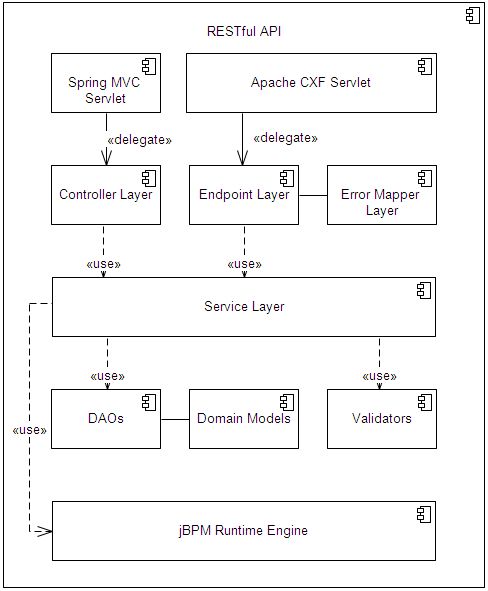
\includegraphics[width=12cm]{figures/restful_api_architecture.png}
	  	\caption{RESTful API internal architecture}
	\end{figure}
	
	Having two different servlets defined does not mean that RESTful API has duplicities. It was necessary to enable
	various capabilities and each required different approach. Both are then allowed to use the same application layers -
	Model in MVC pattern.
	
	\section{Security}\label{sec:security}
	
	RESTful API is tightly coupled with Spring ecosystem in general and heavily uses its features. Often even extends its
	implementations with custom ones. Spring framework is nicely modular and Maven enables to add only those dependencies
	that are really needed. Spring Security library is one of them.
	
	It is an authentication and access-control framework, which became standard for securing Spring-based applications.
	Enabling Spring Security for Spring application is just a matter of adding a simple filter definition to a
	\textbf{web.xml} descriptor file:
	
	\begin{lstlisting}[tabsize=2]
	<filter>
		<filter-name>springSecurityFilterChain</filter-name>
		<filter-class>
			org.springframework.web.filter.DelegatingFilterProxy
		</filter-class>
	</filter>
	<filter-mapping>
		<filter-name>springSecurityFilterChain</filter-name>
		<url-pattern>/*</url-pattern>
	</filter-mapping>
	\end{lstlisting}
	
	\subsection{Authentication}
	
	Further configuration of Spring Security is exclusively defined via Spring context configuration. In RESTful API a file
	found in META-INF/spring/\textbf{spring-security.xml}. Each CXF endpoint has a \textbf{filter chain} defined. Such
	definition example may be:
	
	\begin{lstlisting}[tabsize=2]
	<bean id="springSecurityFilterChain" 
			class="org.springframework.security.web.FilterChainProxy">
		<constructor-arg>
			<list>
				<security:filter-chain pattern="/services/user/identity"
					filters="sessionAuthenticationFilter,\
					basicAuthenticationFilter,anonymousAuthFilter,\
					exceptionTranslationFilter" />
				<security:filter-chain pattern="/services/admission"
					filters="sessionAuthenticationFilter,\
					anonymousAuthFilter,exceptionTranslationFilter" />
			</list>
		</constructor-arg>
	</bean>
	\end{lstlisting}
	
	The above shows two different filter chains that can be found in RESTful API. The first one is used in only one case -
	a UserIdentity was requested via credentials: 
	
	\begin{itemize}
		\item\label{itm:sessionAuthenticationFilter} \textbf{sessionAuthenticationFilter}

		RESTful API's custom authentication filter. It looks for \textbf{X-CTU-FIT-Admission-Session} HTTP request header,
		where a \textbf{session identifier} from \textbf{/user/identity} RESTful API's call is provided. This carries
		information about \textbf{UserIdentity}, its \textbf{Roles}, session validity, \ldots 
		\item \textbf{basicAuthenticationFilter}
		
		Default Basic HTTP Authentication implementation from Spring Security. Verifies \textbf{username} and
		\textbf{password} against Faculty's \gls{LDAP} for employees or RESTful API's database for imported
		\textbf{Admissions}. During the import, \textbf{UserIdentity} is created for each \textbf{Admission}.
		\item\label{itm:anonymousAuthFilter} \textbf{anonymousAuthFilter}
		
		A fallback filter, which sets \textbf{Anonymous Identity} into Security Context, when no \textbf{Identity} has been
		set by previous members of the filter chain.
		\item\label{itm:exceptionTranslationFilter} \textbf{exceptionTranslationFilter}
		
		Translates an Exception thrown during security filter chain processing into HTTP response if possible. 
	\end{itemize}
	
	The later one is a standard security filter chain used for every other use case in RESTful API:
	
	\begin{itemize}
		\item \textbf{sessionAuthenticationFilter}
		\item \textbf{anonymousAuthFilter}
		\item \textbf{exceptionTranslationFilter}
	\end{itemize}
	
	Basically, it is missing \textbf{basicAuthenticationFilter} and therefore it requires RESTful API's session identifier
	to successfully authenticate \textbf{UserIdentity}.
	
	\subsection{Authorization}
	
	To be authenticated is not enough to use any of RESTful API's endpoints. Successful authentication prevents one from
	receiving 401 HTTP response. Each endpoint's call requires a specific \textbf{Permission}. Relationship between
	\textbf{Role} and \textbf{Permission} is M:N. Relationship between \textbf{Role} and \textbf{UserIdentity} is M:N.
	
	Without necessary \textbf{Roles}, authenticated \textbf{UserIdentity} lacks \textbf{Permissions} and such call
	will be rejected with HTTP 403 response.
	
	Endpoint's implementation methods are annotated with \textbf{@Secured} annotations, where required \textbf{Permissions}
	are specified:
	
	\lstset{language=Java}
	\begin{lstlisting}[tabsize=2]
	@Secured("PERM_WRITE_ADMISSION")
	@Consumes({ MediaType.APPLICATION_JSON,
			MediaType.APPLICATION_XML })
	@POST
	@Override
	public Response addAdmission(Admission admission) {
		validateAndDeduplicateAndStore(admission);
		return Response.created(...).build();
	}
	\end{lstlisting}
	
	The example above shows the \textbf{/admission} POST method. It is able to consume both, JSON and XML request body,
	expects \textbf{Admission} serialized object in it and requires the \textbf{PERM\_WRITE\_ADMISSION}
	\textbf{Permission}.
	
	\section{jBPM}
	
	jBPM processing machine luckily integrates with Spring quite well. In RESTful API is configured directly via Spring
	Context and its configuration is stored in \textbf{src/main/resources/META-INF/spring/jbpm.xml}.
	
	Admission business processes and its Use Cases can be simply modelled in BPMN 2.0 using a graphic tool. JBoss Community
	offers such application as Eclipse IDE plugin. All \textbf{.bpmn} processes in RESTful API have been created this way.
	
	\newpage
	\begin{figure}[h]
		\label{fig:eclipse_drools}
	  	\centering
	    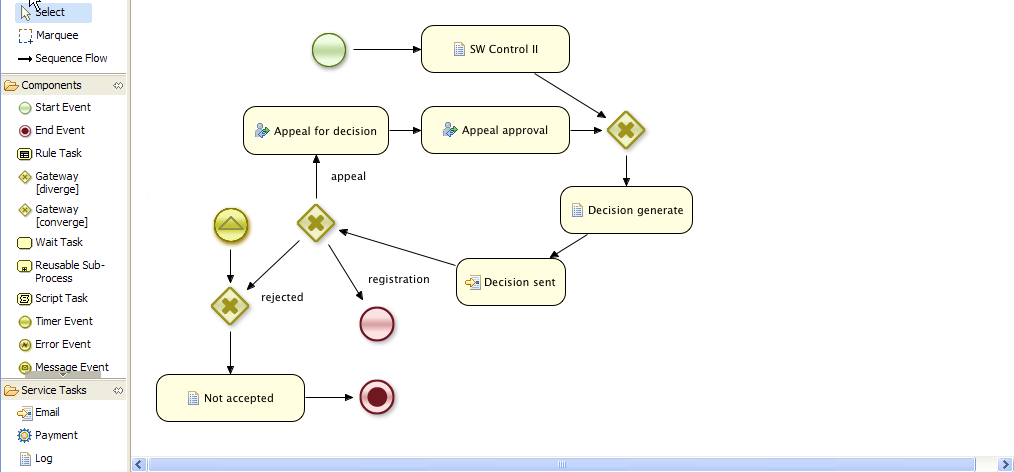
\includegraphics[width=12cm]{figures/eclipse_drools}
	  	\caption{Eclipse Drools BPMN 2.0}
	\end{figure}
	
	It is needed to differentiate between \textbf{bachelor's} and \textbf{master's} Admission processes. These are further
	split into smaller parts like registration, apology, enrollment, \ldots - also BPMN 2.0 processes. Their \textbf{.bpmn}
	representations are located in \textbf{src/main/resources/bsp} respectively \textbf{src/main/resources/msp}
	directories. Common processes are then stored in \textbf{src/main/resources/process} project directory. Their graphical
	forms can be found in Appendices section \ref{app:jbpm}.
	
	Each RESTful API call, which has some impact on Admission process should invoke appropriate task in jBPM runtime
	engine. Such action is allowed by using Spring managed \textbf{@Service} annotated implementations from
	\textbf{cz.cvut.fit.mi\_mpr\_dip.admission.jbpm} package. After RESTful API's Service and DAO layers finish their job,
	Admission is then further passed to jBPM runtime engine for evaluation. This guarantees correct state in Admission
	process.
	
	In Admission object representation, which RESTful API provides to its consumers, a state is represented by
	AdmissionState object. Modification of the state is jBPM runtime engine's responsibility. Further it handles a few
	other tasks including notification via e-mail and writing an information about changes made to the Admission object in
	logs.
	
	\section{Error handling}
	
	JAX-RS itself defines error mapping interfaces and a framework for capturing exceptional states. Apache CXF, used as
	implementation of JAX-RS in RESTful API, handles several common errors such as authentication, authorization and bad
	request body format. Returns appropriate response, when error mapper is registered. CXF servlet has to be configured to
	do so:
	
	\lstset{language=XML}
	\begin{lstlisting}[tabsize=2]
	<jaxrs:server id="restContainer" address="/">
		...
		<jaxrs:providers>
			...
			<ref bean="accessDeniedExceptionMapper" />
			<ref bean="businessExceptionMapper" />
			<ref bean="technicalExceptionMapper" />
			<ref bean="jaxbExceptionMapper" />
			<ref bean="webApplicationExceptionMapper" />
			<ref bean="throwableExceptionMapper" />
		</jaxrs:providers>
	</jaxrs:server>
	\end{lstlisting}
	
	All \textbf{ExceptionMapper} Spring managed beans are implementations of
	\textbf{javax.ws.rs.ext.ExceptionMapper\textless{E}\textgreater} interface, where \textbf{E} is a subclass of
	\textbf{java.lang.Throwable} being captured by this Exception Mapper.
	Besides special types of Exceptions defined by various frameworks:
	
	\begin{itemize}
		\item \textbf{AccessDeniedException}
		
		Typically produces HTTP 401 or 403 response
		\item \textbf{JaxbException}
		
		Produces HTTP 400 response
		\item \textbf{WebApplicationException}
		
		Various 4xx and in some special cases 5xx HTTP response
	\end{itemize}
	
	RESTful API defines three \uv{levels} of custom Exceptions, which are either thrown by Validation layer or some library
	used by RESTful API:
	
	\begin{itemize}
		\item \textbf{BusinessException}
		
		Exclusively thrown in Validation layer. This means an error on Client side. Request constrains are violated, Client
		is not authorized, \ldots Produces 4xx HTTP response and results in \verb|OK|\footnote{RESTful API did not produce
		any errors on server side. Client has supplied invalid request and typically by fixing problem on his side, request
		can be accepted and could result in 2xx or 3xx HTTP response.} RESTful API status.
		\item \textbf{TechnicalException}
		
		A known and recognized Exception, which is usually a wrapper for the original Exception thrown by a backend or
		database. In this case a Client cannot fix the problem on his side, but he can retry later - a cause of the problem
		is shown in the response message. Usually returns HTTP 500 response.
		\item \textbf{Throwable}
		
		An unexpected and unknown error. Most probably indicates a bug in RESTful API. Results in HTTP error 500 without
		further description as it may put some Java specific information into the message.
		
		Both TechnicalException and Throwable cause \verb|ERROR|\footnote{An error has occurred on Server side and Client
		cannot fix it by changing his request. ERROR status forces RESTful API's Logging service to be more verbose than OK
		status. It writes full Exception chain stack trace into server log with ERROR priority.} RESTful API response status.
	\end{itemize}
	
	A standardized Error Response body is used for all Exceptional states of RESTful API:
	
	\begin{lstlisting}[tabsize=2]
	<errorResponse>
		<message>Access is denied</message>
		<internalRequestId>
			33d91c25-9d42-4291-9af7-a387dbb49ffe
		</internalRequestId>
	</errorResponse>
	\end{lstlisting}
	
	From which:
	
	\begin{itemize}
		\item \textbf{message}
		
		Should tell the Client what happened, if possible.
		\item \textbf{internalRequestId} 
		
		A value generated for each RESTful API request and is its unique identifier, which is further appended to each row in
		the server log and so progress can be easily traced in it.
		Non ERROR responses contain this value in HTTP response headers.
	\end{itemize}
	
	\section{Profiling, Logging}

	An important part of business logic of each application should be its ability to inform system administrator, operation
	or even developer, what is happening and in a case of failure, why it was not able to process the task.
	
	RESTful API does not have many possibilities to choose from. Writing a system log seems to be a simple and usable
	approach.
	
	As I already mentioned, SLF4j logging API and Logback as its implementation is used. To utilize their capabilities,
	RESTful API defines and implements \textbf{LoggingService} interface. This service contains:
	
	\begin{itemize}
		\item \textbf{logRequest(BufferedRequestWrapper httpRequest)}
		
		All information from HTTP request including headers
		\item \textbf{logRequestBody(BufferedRequestWrapper httpRequest)}
		
		Copies HTTP request body InputStream and sends to Logger
		\item \textbf{logResponse(BufferedResponseWrapper httpResponse)}
		
		All information from HTTP response including headers and \textbf{status} - OK, request processing duration, HTTP
		response code
		\item \textbf{logResponseBody(BufferedResponseWrapper httpResponse)}
		
		Copies HTTP response body OutputStream and sends to Logger
		\item \textbf{logErrorResponse(BusinessException exception)}
		
		The same as \textbf{logResponse}
		\item \textbf{logErrorResponse(TechnicalException exception)}
		
		The same as \textbf{logResponse}, but the \textbf{status} is ERROR and Exception's stack trace is sent to the Logger
		\item \textbf{logErrorResponse(Throwable throwable, Integer httpResponseCode)}
		
		The same as logErrorResponse(TechnicalException exception), but \textbf{UnexpectedError} message is put into the
		response body
	\end{itemize}

	LoggingService methods are executed from \textbf{LoggingFilter}, which is an implementation of a standard
	\textbf{javax.servlet.Filter}. A single exception is executing \textbf{logErrorResponse} methods, which are invoked
	from JAX-RS Exception Mappers.
	
	To put it all together one example RESTful API successful call results in these log entries:
	
	\begin{verbatim}
	12-06-26 11:14:19.618 INFO  991a0741-d86b-4334-8134-876c5ad25967 
	admission-request 
	call-identifier=/admission/services/user/identity_GET 
	Connection=keep-alive Authorization=Basic_bGVzczpsZXNz== 
	Accept=application/xml User-Agent=Java/1.7.0_05 
	Host=localhost:9090 query=null
	12-06-26 11:14:19.633 INFO  991a0741-d86b-4334-8134-876c5ad25967 
	admission-request-body
	12-06-26 11:14:19.846 INFO  991a0741-d86b-4334-8134-876c5ad25967 
	c.c.f.m.a.a.UserIdentityAuthenticationProvider 
	Found authenticationService 
	[c.c.f.m.a.s.a.LdapAuthenticationService] for authentication 
	[LDAP]
	12-06-26 11:14:19.846 INFO  991a0741-d86b-4334-8134-876c5ad25967 
	c.c.f.m.a.a.UserIdentityAuthenticationProvider 
	Successfuly authentified [less]
	12-06-26 11:14:20.638 INFO  991a0741-d86b-4334-8134-876c5ad25967 
	admission-response 
	call-identifier=/admission/services/user/identity_GET code=200 
	duration=1024 status=OK
	12-06-26 11:14:20.638 INFO  991a0741-d86b-4334-8134-876c5ad25967 
	admission-response-body <?xml version="1.0" ...
	\end{verbatim}
	
	Each log entry contains a timestamp, \textbf{internalRequestId}, Logger name (admission-request,
	admission-request-body, \ldots) followed by information being logged, which can contain more parts separated by a
	single white space.
	
	It is a custom that application server with JEE application deployed is \uv{hidden} behind AJP or HTTP proxy, e.g.
	Apache httpd or nginx. These applications also provide some logging and profiling functionality, but to enable RESTful
	API's profiling capabilities, \textbf{duration} in ms is also sent to Logger.
	
	Logback is further configurable and allows many different log formats, outputs, log rotating etc. File log appender is
	used in production environment. Console output is configured for development.
	
	One important information is that the entire logging and file writing process is asynchronous and so it does not block
	RESTful API from completing its primary task. This is why under a high load with many concurrent users log entries
	might appear in different order than expected. However, it is very common in all enterprise production environments.
